\chapter{Results} \label{study_results}

This Chapter describes all the results gathered throughout the study. They are presented accordingly to the method used and for each one of them I reported the raw numbers and relevance with respect to the RQs.

As a final not, due to confidentiality issues it was not possible to report the raw data. For this reason, as briefly explained in the previous Chapter, all the sensitive information has been eliminated and anonymized.



\section{Informal Interviews}
As mentioned in the Data Gathering section the informal interviews conducted within this study helped to narrow the scope of the study itself and to gain knowledge of important problems faced by testers along the time frame of this study.

Furthermore, given the randomness associated with this method I will only report the topics covered in such conversations. Moreover, due to confidentiality and anonymity, I am not allowed to report most of the literal quotations that are of interest for this study.

The topics covered, during such interviews are reported in Table \ref{tab:informal_interviews_topics}. For completeness's sake I also included the date and the approximate length of these conversations.

		\begin{table}[htb]
			\centering
			%\renewcommand{\arraystretch}{1.2}
			\caption{Topics covered while performing the Informal interviews}
			\label{tab:informal_interviews_topics}
			\begin{tabulary}{\columnwidth}{|L|L|L|}
				\hline
				
				\textbf{Date} {\tiny (YYYY/MM/DD)} & \textbf{Approx. duration} & \textbf{Topics covered} \\
				\hline
				
				2015/02/15 &
				10 min. &
				- How does the test pipeline works.\newline
				- Recurrent problems with high level tests. \\
				\hline
				
				2015/02/18 &
				10 min. &
				TO be completed\\
				\hline
				
                
			\end{tabulary}		
		\end{table}


\section{Mining of the Forum}
The process explained in Section \ref{mining_forum} yielded 15 possible interesting documents. Those are in various formats, spacing from actual entries in the forum to pictures of whiteboards taken during workshops.

Some of these documents are central to this study, whereas others only highlight problems that are platform or tool specific. For transparency's sake I also reported these entries, but they were not used in the \textit{theory generation} step.

\begin{figure}[ht]
    \centering
    \begin{minipage}[t]{0.45\linewidth}
        \centering
        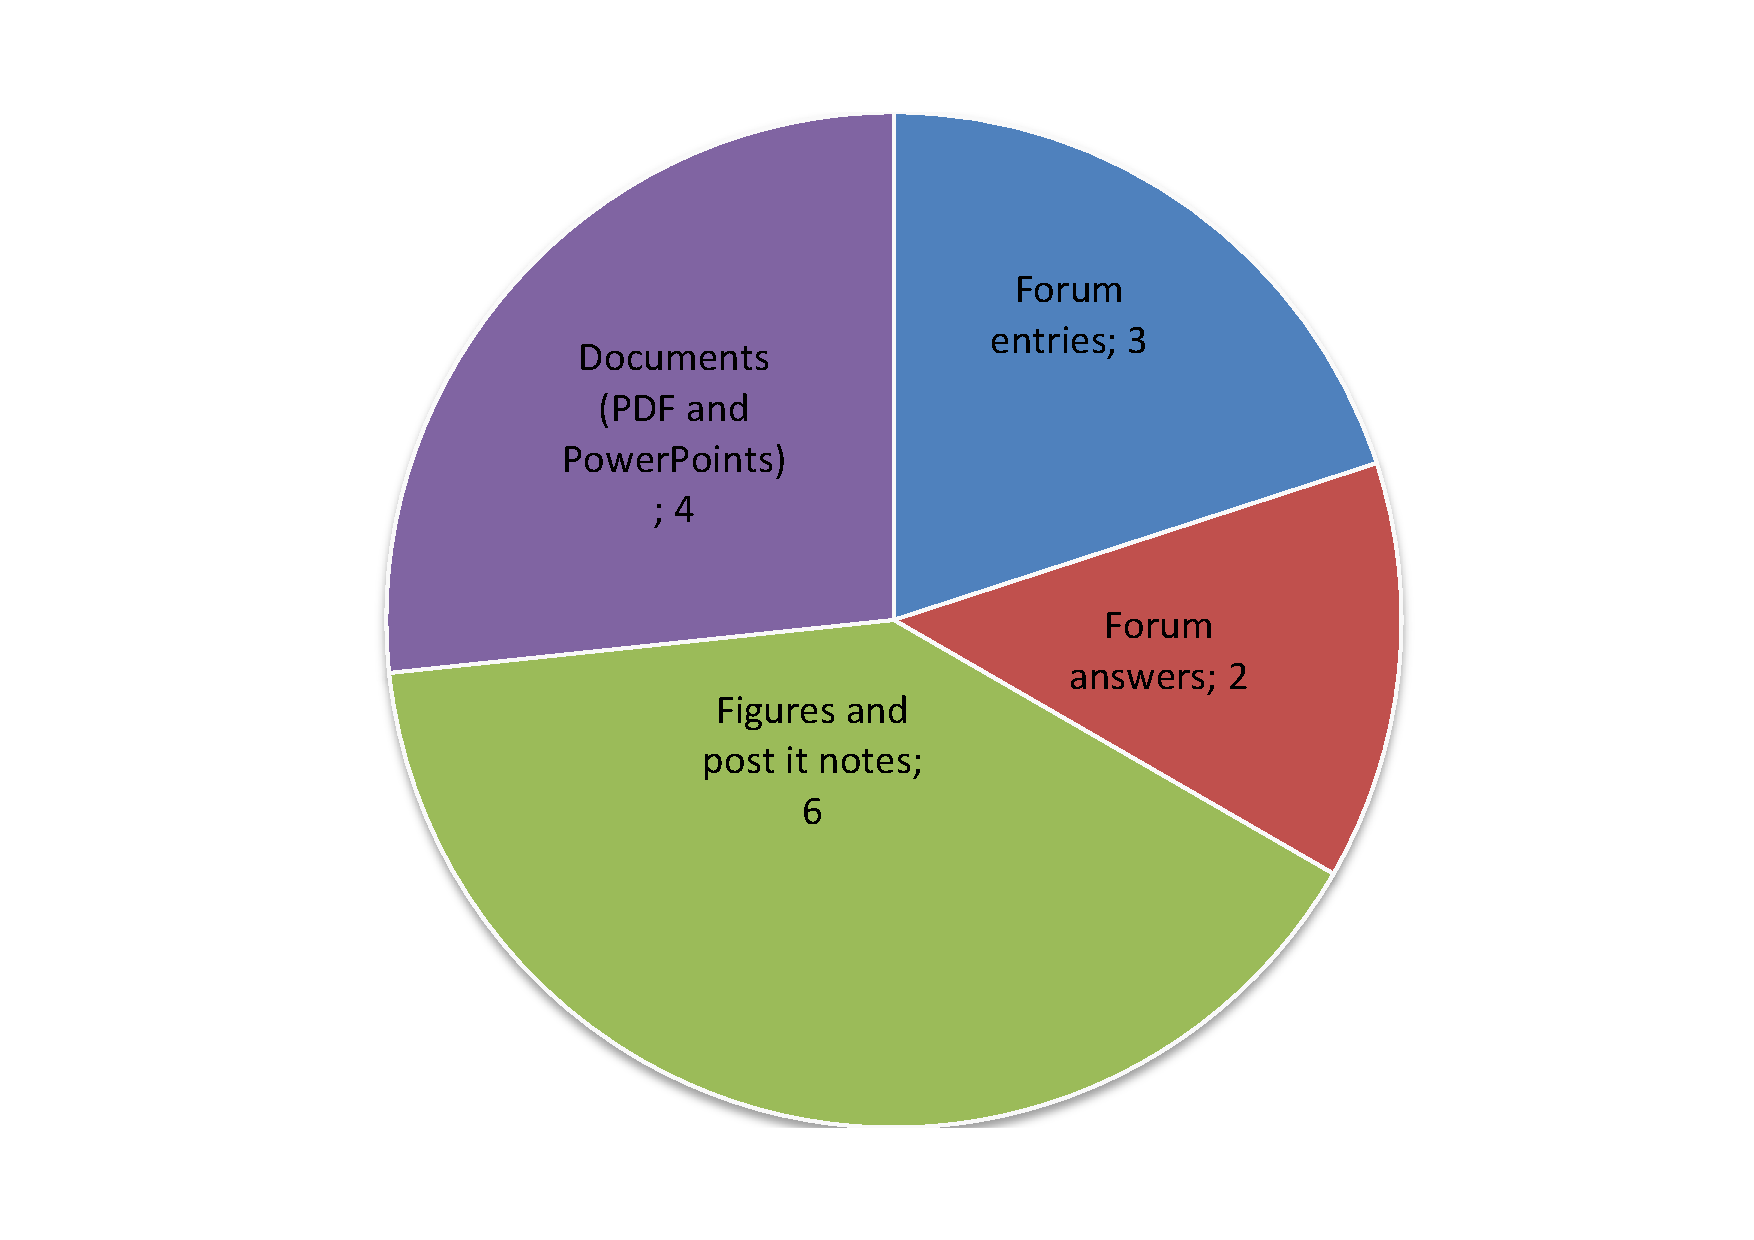
\includegraphics[width=\textwidth]{figure/results/confluence_doc_types}
        \caption{Type of the results yielded by the forum's mining}
        \label{fig:confluence_types}
    \end{minipage}
    \hspace{0.5cm}
    \begin{minipage}[t]{0.45\linewidth}
        \centering
        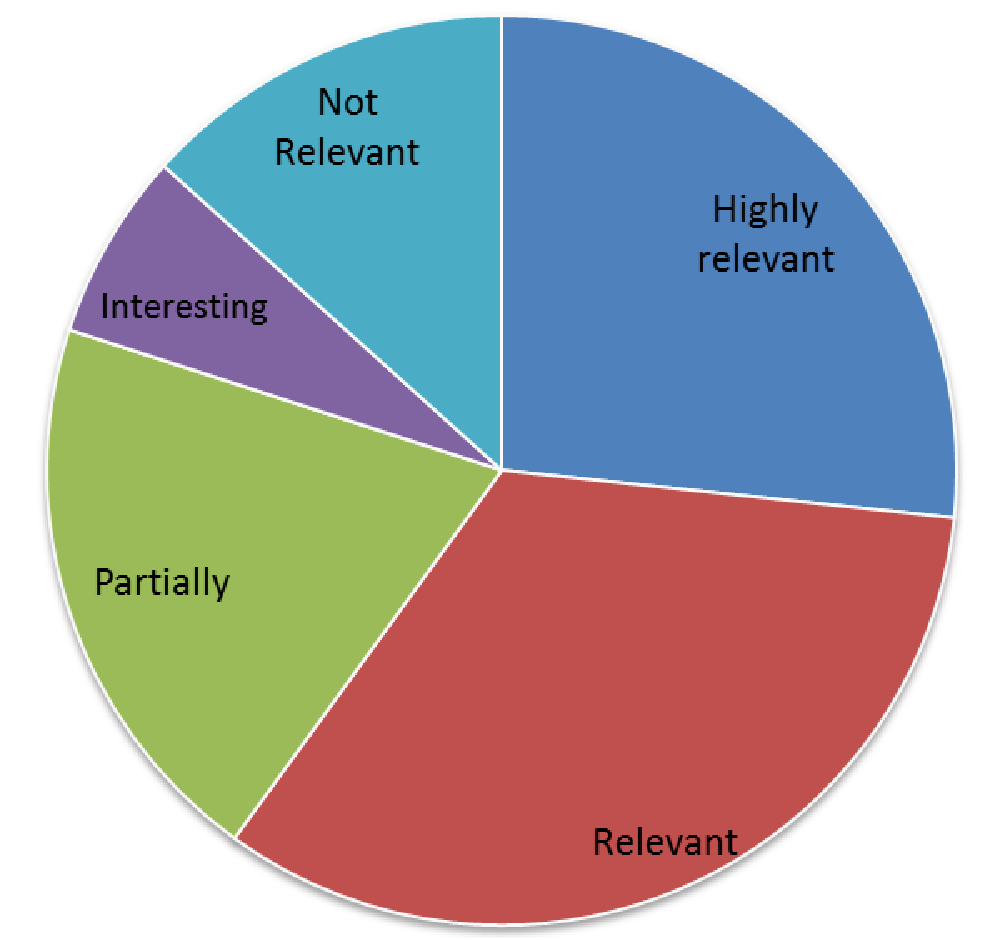
\includegraphics[width=\textwidth]{figure/results/confluence_doc_relevance}
        \caption{Relevance of Confluence entries according to the RQs defined in this study}
        \label{fig:confluence_relevance}
    \end{minipage}
\end{figure}


%Their type is summarized in Img. \ref{img:mining_confluence}.

\todo{Improve readibility of figures \ref{fig:confluence_types},\ref{fig:confluence_relevance}
}

\section{Mining of the Issue Tracer / Backlogs}


\section{Analysis of the Repositories}

\section{Semi-Structured Interviews}